% $Id: power-of-test.tex,v 1.20 2006/05/11 22:08:27 hana Exp $

\section{Evaluation of the Tests}
\label{sec:power}
%
In this section we examine the question of
whether these tests are powerful enough for our 
real-world usage.  Do they detect bugs when they should?  Will these tests do 
better than our problematic \emph{ad hoc} tests that were failing frequently 
even though the code was correct?

In statistical hypothesis testing, two types of errors can arise.  A type I
error occurs if the null hypothesis is rejected when it is true. A type II
error occurs if the null hypothesis is accepted when it is false. 
In our framework, the
consequence of a type I error is that the unit test fails
even if the code is correct. A type II error means that the unit test does
not fail even when the program contains errors. 

In this section we investigate the behavior of the tests described in
Section~\ref{sec:statform} in terms of the two types of errors. We consider
two different tests, one suited for modeling by the Poisson distribution and
one with normal distributed values.  We assess the probability of type I and
type II errors by repeating the stochastic tests $1000$ times.

The first test (denoted as T1) corresponds to the location choice
model described in Section~\ref{sec:example}, where we vary its input
parameters (number of agents, number of locations $K$, number of repetitions
$R$).

The second test (denoted as T2) runs our \emph{Household Transition} model that removes a
certain number of households from the existing set of households (thus,
simulating deaths and emigration in a given region). The households to be
removed are selected randomly while preserving specific characteristics of the
total set. We consider four income categories, from each of which a given
number of households is removed. The test checks if after running the model
the average age of households for each income category remains the same.

Figure~\ref{fig:error1} shows the frequency of type I error in T1 and T2 as a
function of $R$ for two different significance levels $\alpha$. Note that
since the outputs from T2 are continuous, the Poisson tests are not applicable
here. The ideal behavior is when the frequency is equal to $\alpha$ (marked by
a dashed line). It can be seen that the likelihood-ratio test for normally
distributed data for T1 is far from $\alpha$, whereas the both Poisson tests
are close to the $\alpha$ level. These results suggest that the outputs of our
example T1 are better modeled by Poisson distribution.  Furthermore, it can be
seen from the figure that increasing the number of replicates $R$ does not
considerably influences the frequency, if the data of T1 are modeled by
Poisson distribution. This means that tests with a relatively small number of
replicates, such as 10, are sufficient for minimizing the occurrence of type I
errors. In this experiment, we used $1000$ agents and number of locations
$K=50$ for T1. Also, a square root transformation was applied to the outputs
in order to obtain $LRTS_{normal}$ for this test. T2 was run with removing
$2000$ households from existing $5000$ households and no transformation was
performed.

\begin{figure}[t]
\begin{center}
\includegraphics[angle=-90, scale=0.3]{error1.ps}
\caption{\label{fig:error1} \small Frequency of a type I error for tests T1
  and T2 obtained with different test statistics. Two levels of significance
  are used: $\alpha=0.05$ (left panel)
  and $\alpha=0.01$ (right panel). }
\end{center}
\end{figure}

In Figure~\ref{fig:error1-k-agents}, the same frequency for T1 and the two
Poisson tests is shown as a function of $K$\@.  It can be seen that both tests
are independent of the number of dimensions. This implies
that tests with a small number of dimensions (for example up to 10), are sufficient for
minimizing the occurrence of type I errors. Note that in this experiment, the
ratio of number of agents per location was kept constant, namely 20.


 \begin{figure}[t]
\begin{center}
  \includegraphics[angle=-90, scale=0.2]{error1_k_agents.ps}
\caption{\label{fig:error1-k-agents} \small Frequency of type I error for T1 as a
  function of $K$ (number of locations) on a log scale.  The significance
  level is set to $\alpha=0.05$ (dashed line) and the number of replicates is
  $R=10$.}
\end{center}
\end{figure}
 
The frequency of type II errors are usually expressed by the power function.
The power function is defined as the probability that the null hypothesis is
rejected when it is false. Thus, the ideal power approaches 1.
Figure~\ref{fig:power-T1} shows the power function for T1 for $\alpha=0.05$
and $\alpha=0.01$. The number of locations is $K=50$ and number of agents is
$1000$. In each run of this experiment there was a few agents added to one
of the more expensive locations and thus, the mean of the distribution of that
location was increased which made the null hypothesis false. The number of
agents that were added is plotted on the $x$ axes of the figure. Note that
the expected value for that location is $5.8$. Intuitively, the larger the
increment (and thus the larger the deviation from the expected value), the
better the power.  Also, the larger the number of replicates $R$, the better
the power. The plots reveal that in terms of power, the Pearson test
statistic is vastly inferior to the $LRTS_{poisson}$ when the number of
replicates is larger than 2, and thus we recommend using
$LRTS_{poisson}$ when dealing with Poisson data.

 \begin{figure}[t]
\begin{center}
  \includegraphics[angle=-90, scale=0.3]{power_poisson.ps}
\caption{\label{fig:power-T1} \small Power curves for $\alpha=0.05$ (left panel)
  and $\alpha=0.01$ (right panel) for the test T1. Power based on $LRTS_{poisson}$ is
  marked by solid lines and labeled as LR($R$) where $R$ is the number of
  replicates. Power based on Pearson test statistics is marked by dashed lines
  and labeled as Pe($R$). The x-axes show the number of agents that were added
  in each iteration to the results in one of the more expensive locations (the
  expected value of that location is $5.8$ agents). The number of dimensions
  is $K=50$.}
\end{center}
\end{figure}

Figure~\ref{fig:power-T2} shows power curves for the test T2 based on
$LRTS_{normal}$.  In this case, we increased the average age of one income
category by increments (approximately of size one variance) marked on the $x$
axes. As in the case of T1, the power increases with increasing deviation from
the expected value and with increasing number of replicates $R$. Note that
since we are dealing with only four dimensions (in contrast to 50 in case of
T1), it is easier to detect deviation, and therefore the overall level of the
power is higher than in Figure~\ref{fig:power-T1}.  This means that tests with
fewer dimensions are preferable in order to detect errors in the code.

\begin{figure}
\begin{center}
  \includegraphics[angle=-90, scale=0.3]{power_normal.ps}
\caption{\label{fig:power-T2} \small Power curves for $\alpha=0.05$ (left panel)
  and $\alpha=0.01$ (right panel) for the test T2 based on LRTS for normal
  distribution.  The x-axes show age added in each iteration to the
  average age of agents of one income category. The number of dimensions is
  $K=4$.}
\end{center}
\end{figure}
% \begin{figure}
% \centering
% \centerline{\pdfimage width 2.0in {test.pdf}}
% \caption{A sample graphic (.pdf format).}
% \end{figure}

% LocalWords:  UnitTests LandPriceModel UnitTest tex hana LRTS poisson Pe

%%% Local Variables: 
%%% mode: latex
%%% TeX-master: "main"
%%% End: 
